\section{Water-to-Water Heat Pump Parameter / Coefficient Generator (Cooling and Heating Mode)}\label{water-to-water-heat-pump-parameter-coefficient-generator-cooling-and-heating-mode}

This document gives brief instructions on generating the parameters/ coefficients for the water-to-water heat pump models in cooling and heating mode. The Excel\textsuperscript{TM}\ spreadsheets (WaterWater\_PE\_Cooling.xls and WaterWater\_PE\_Heating.xls) are used. Since the spreadsheet functions are very similar for both cooling and heating modes, only one instruction document is supplied. The spreadsheet generates:

\begin{itemize}
\item
  parameters for the parameter estimation based model.
\item
  coefficients for the curve-fit model.
\end{itemize}

The following theses have detailed information about the curve-fit model and parameter estimation based model:

Jin, Hui. 2002. Parameter Estimation Based Models of Water Source Heat Pumps. Phd. Thesis, Department of Mechanical and Aerospace Engineering, Oklahoma State University. (downloadable at \href{http://www.hvac.okstate.edu}{www.hvac.okstate.edu})

Shenoy,Arun. 2004. Simulation, Modeling and Analysis of Water to Air Heat Pump. M.S. Thesis, Department of Mechanical and Aerospace Engineering, Oklahoma State University. (downloadable at \href{http://www.hvac.okstate.edu}{www.hvac.okstate.edu})

Tang,C.C. 2004. Modeling Packaged Heat Pumps in a Quasi-Steady State Energy Simulation Program. M.S. Thesis, Department of Mechanical and Aerospace Engineering, Oklahoma State University. (downloadable at \href{http://www.hvac.okstate.edu}{www.hvac.okstate.edu})

\subsection{Step 1: Catalog Data Input}\label{step-1-catalog-data-input-001}

Data points are obtained from the heat pump manufacturer data. Minimum data points for the parameter estimation based model are 32 data points according to Jin (2002). The curve-fit model performance is not affected by the number of data points and a minimum of 5 data points is required since the governing equations require 6 coefficients. The data points must have varying inlet conditions (e.g.~water flow rates, inlet water temperatures, etc.) that covers the entire range of the heat pump operating conditions. Correction tables provided by the manufacturer should be used to extend the catalog data range in order to have a good set of parameters/coefficients.

\begin{itemize}
\item
  Using the heat pump performance data, enter the values to Table~\ref{table:comparison-of-ee-with-esp-rdoe-2blast-weather} in worksheet ``CATALOG DATA''. The values can be in SI or IP units.
\item
  Click on Button 1 based on the units used.
\end{itemize}

For IP units:

\begin{figure}[htbp]
\centering
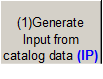
\includegraphics{media/image037.png}
\caption{}
\end{figure}

For SI units:

\begin{figure}[htbp]
\centering
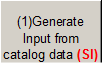
\includegraphics{media/image038.png}
\caption{}
\end{figure}

\begin{itemize}
\item
  The program will convert the values to the desired units and display them on Table~\ref{table:input-file-extensions-with-implied-data-types} in worksheet ``INPUT''.
\item
  The button shown below is used clearing Table~\ref{table:comparison-of-ee-with-esp-rdoe-2blast-weather} (worksheet ``CATALOG DATA''), and Table~\ref{table:input-file-extensions-with-implied-data-types} (worksheet ``INPUT''). It is advisable to clear the tables before generating parameters/coefficients for a new heat pump model.
\end{itemize}

\begin{figure}[htbp]
\centering
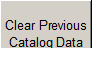
\includegraphics{media/image039.png}
\caption{}
\end{figure}

After Table~\ref{table:input-file-extensions-with-implied-data-types} is created, the parameters/coefficients are then calculated as follows:

\begin{itemize}
\item
  Worksheet ``ParamEstimator'' is used for generating the parameters for the parameter estimation based model using Nelder Mead Simplex. Refer to the steps in the Parameter Estimation Procedure.
\item
  Worksheet ``CoeffCalculator'' is used for calculate the coefficients for the curve-fit model using the generalized least square method. Refer to the steps in the Curve Fit Model procedure.
\end{itemize}

\subsection{Parameter Estimation Procedure}\label{parameter-estimation-procedure-001}

\subsubsection{Step 2a: Generating First Set of Parameters (PE-Based Model)}\label{step-2a-generating-first-set-of-parameters-pe-based-model-001}

\begin{itemize}
\item
  Using Table~\ref{table:input-file-extensions-with-implied-data-types}, the program can generate parameters. The user must fill all the cells colored light blue in worksheet ``ParamEstimator''.
\item
  \textbf{Accuracy:} Start with a low accuracy for faster convergence, recommended value of 0.001.
\item
  \textbf{Compressor Type:} Only reciprocating compressor is currently available in EnergyPlus. One might be able to generate parameters for heat pump model with different compressor types but this might result in unrealistic parameters.
\item
  \textbf{Refrigerant:} Contact the manufacturer on the refrigerant used to generate the catalog data and select from the list of refrigerants. Usually the refrigerant used is R22. .
\item
  \textbf{Which Initial Guess?:} The user may choose a set of initial guesses(1-5) that will be used by the optimization routine in generating the parameters. Start with 1, which is the set of initial guess 1 at column B.
\item
  \textbf{Initial Guess:} Initial guess for all the parameters. For Initial Guess 1, enter a value of 1 for all the parameters except for the loss factor (less than 1.0). The loss factor should be less than 1.0 because the efficiency of the compressor should be less than 100\%. Adjust the values in Initial Guess 1 if the program happens to crash and try again.
\item
  Now click on Button 2 shown below to generate the parameters.
\end{itemize}

\begin{figure}[htbp]
\centering
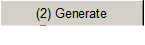
\includegraphics{media/image040.png}
\caption{}
\end{figure}

It will take some time to generate the parameters depending on the number of data points. The parameters generated will be displayed at Parameters 1.

\begin{itemize}
\item
  Look at the error analysis of Error 1 which gives the user a summary of the errors for Qload, Qsource and Power. An average error of 5-8\% is achievable for all the values.
\item
  The errors for all the individual catalog data points are displayed in worksheet ``RESULT''.
\end{itemize}

\subsubsection{Step 2b: Improving the Set of Parameters (PE-Based Model)}\label{step-2b-improving-the-set-of-parameters-pe-based-model-001}

\begin{itemize}
\item
  After the initial set of parameters has been generated, the user can increase the accuracy of the parameters by using parameters generated as the initial guess for the second simulation and increasing the accuracy of the program.
\item
  Copy and Paste Parameters 1 to Initial Guess 2.
\item
  Change the initial guess indicator (\textbf{Which Initial Guess?:)} from 1 to 2.
\item
  Increase the accuracy by twice. For example, set accuracy to 0.000001.
\item
  Now click on Button 2 shown below to generate the second set of parameters.
\end{itemize}

\begin{figure}[htbp]
\centering
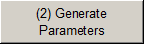
\includegraphics{media/image041.png}
\caption{}
\end{figure}

The simulation time would most likely be less but it depends on the accuracy value as well. And the parameters generated will be displayed at Parameter 2.

\begin{itemize}
\item
  Compare Error 2 to Error 1, the error values should be less which means that the parameters are getting better and more accurate.
\item
  Repeat the steps in 2a and 2b until a desired set of error values is achieved or the errors stop decreasing
\end{itemize}

\subsubsection{Step 3: Generating EnergyPlus Input Parameters}\label{step-3-generating-energyplus-input-parameters-001}

\begin{itemize}
\tightlist
\item
  Click on the Button 3 shown below to convert and arrange the parameters generated to fit EnergyPlus Input File (IDF) which will be listed from cell B52:B59 for cooling mode and B46:B54 for heating mode.
\end{itemize}

\begin{figure}[htbp]
\centering
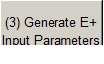
\includegraphics{media/image042.png}
\caption{}
\end{figure}

\begin{itemize}
\tightlist
\item
  The button shown below in worksheet ``ParamEstimator'' is used for clearing Initial Guess (2-5), Parameters(1-5), Error(1-5), EnergyPlus Input parameters and Result(1-5) in worksheet ``RESULT''.
\end{itemize}

\begin{figure}[htbp]
\centering

\includegraphics{media/image043.png}
\caption{}
\end{figure}

\subsection{End Parameter Estimation Procedure}\label{end-parameter-estimation-procedure-001}

\subsection{Curve Fit Model Procedure}\label{curve-fit-model-procedure-001}

\subsubsection{Step 2: Generating the coefficients (Curve-Fit Model)}\label{step-2-generating-the-coefficients-curve-fit-model-001}

\begin{itemize}
\item
  Using Table~\ref{table:input-file-extensions-with-implied-data-types}, the program is ready to generate the coefficients. User is required to fill all the cells colored light blue in worksheet ``CoeffCalculator''.
\item
  \textbf{RatedLoadVolFlowRate:} Rated load side volumetric flow rate (m\(^{3}\)/s) which corresponds to the highest load side heat transfer rate listed in the catalog data.
\item
  \textbf{RatedSourceVolFlowRate:} Rated source side volumetric flow rate (m\(^{3}\)/s) which corresponds to the highest load side heat transfer rate listed in the catalog data.
\item
  \textbf{RatedQload:} Rated load side heat transfer rate (W) which is the highest load side heat transfer rate listed in the catalog data.
\item
  \textbf{RatedPower:} Rated power consumption (W) which corresponds to the highest load side heat transfer rate listed in the catalog data.
\item
  Now click on Button 2 shown below to calculate the coefficients.
\end{itemize}

\begin{figure}[htbp]
\centering
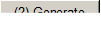
\includegraphics{media/image044.png}
\caption{}
\end{figure}

\begin{itemize}
\item
  The coefficients for the corresponding curves are listed at cell B12:C16. Error analysis of model is listed at cell B19:B27.
\item
  The errors for all the individual catalog data points are displayed in worksheet ``RESULT''.
\item
  The button shown below in worksheet ``CoeffCalculator'' is used for clearing the coefficients, the error analysis and the outputs in worksheet ``RESULT''.
\end{itemize}

\begin{figure}[htbp]
\centering

\includegraphics{media/image045.png}
\caption{}
\end{figure}

\subsection{End Curve Fit Model Procedure}\label{end-curve-fit-model-procedure-001}
